\begin{center}
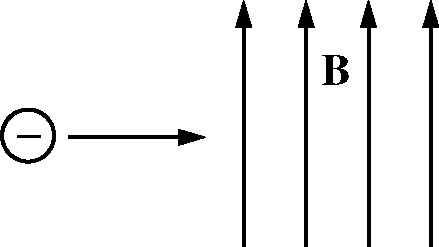
\includegraphics[scale=0.25]{images/img-013-026.png}
\end{center}

% Multiple Choice Question 28
\begin{questions}\setcounter{question}{27}\question
An electron moving to the right with constant velocity enters a region with a uniform magnetic field B directed toward the top of the page, as shown above. In what direction will the electron initially be deflected?

\begin{choices}
\choice Toward the top of the page
\choice Toward the bottom of the page
\choice Into the page
\choice Out of the page
\choice Toward the left
\end{choices}\end{questions}

